In this section will be presented an overview of the user’s interface of the eMALL system. The focus will be mainly on the user experience, secondarily on the user interface, which, although designed with attention to detail, remains subject to changes dependent on testing with focus groups; this is why, the user interface shown below is limited to the desktop browser version, as it allowed us to present both the UI on the CPO side and the EVD side (the CPO side is not available on mobile devices). For the mobile version (both app and mobile browser) it will be sufficient to scale the interface, which in any case is designed to be responsive and therefore scalable regardless of the specifications and type of user.

\section{General Overview}
\label{sec: general_overview}%
The image below shows a map of the pages which can be accessed from the application. All pages can only be accessed from the log-in page (shown below), and works as a page that divides the marketing section (homepage) from the service section (CPO and EVD dashboards). Let's overlook the EVDs registration page mockup, and the businesses login one, as they are very similar, and still standard.

\begin{figure} [H]
	\begin{center}
		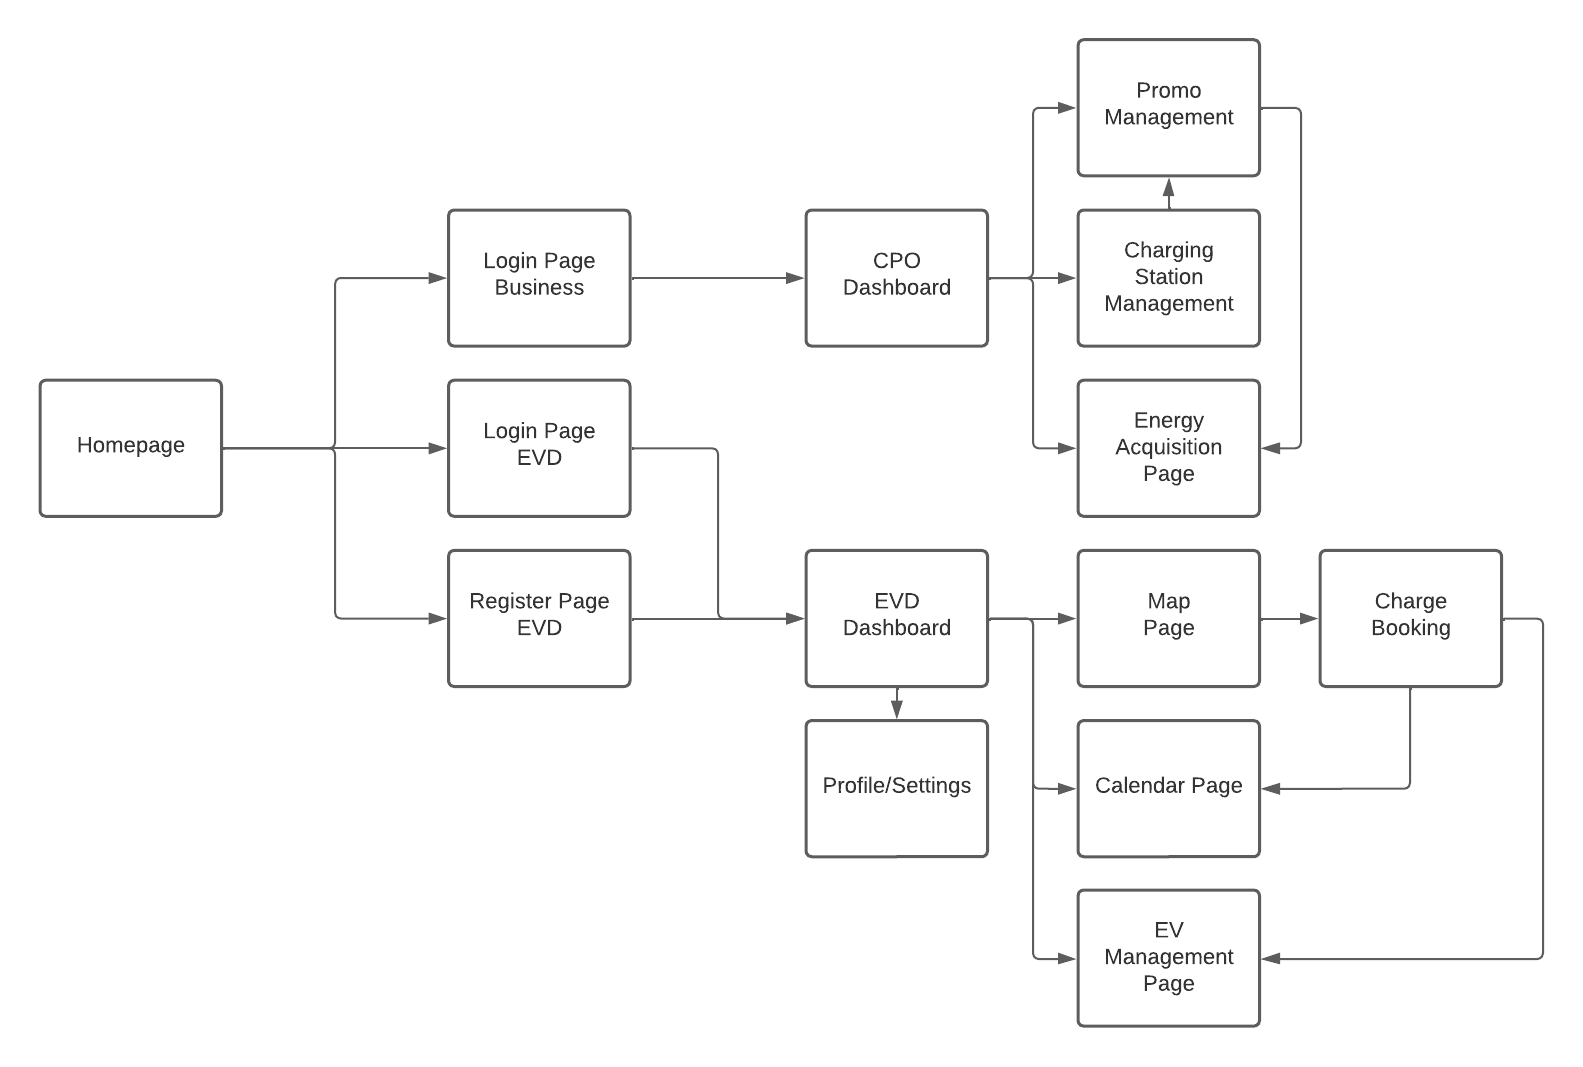
\includegraphics[width=1\linewidth]{UI/Pages}
		\caption{Pages of the eMALL system}
		\label{fig: cd}
	\end{center}
\end{figure}

We’ll also skip the homepage interface, as it is linked to marketing choices (colors, fonts, style) which are neither relevant nor functional to the description of the service.

As previously mentioned, the login section allows you to redirect the user, obviously following a successful login, to the dashboard from which you can access the service and take advantage of its features. There are two types of dashboards, as are two actors involved in the eMALL processes: CPO, and registered EVD, who access the service via two different login pages, one reserved for the public (EVDs), one reserved for CPOs. 

The CPO dashboard is aesthetically different from the EVD dashboard in the choice of colors, but maintains an almost identical structure in order to optimize and simplify its development, which can be reduced to the definition of a few reusable components, following an industrial, scalable design method and easily maintainable over time.

From the CPOs dashboard the following pages can be accessed:

\begin{itemize}
	\item Promo and offers management
	\item Charging stations management
	\item Energy acquisition management (interface with DSO offers)
\end{itemize}

From the EVDs dashboard the following pages can be accessed:

\begin{itemize}
	\item User profile and settings management
	\item Map of charging stations
	\item User’s calendar and appointments booked
	\item Owned EVs management
	\item Booking charge
\end{itemize}

It is also possible to receive targeted notifications for the user. All of the pages illustrated above are described in detail in the following pages. Any interactive panel and dialog is neglected in the user interfaces presented.

Any interactive panels and dialogs are neglected in the development of the interface.

\begin{figure} [H]
	\begin{center}
		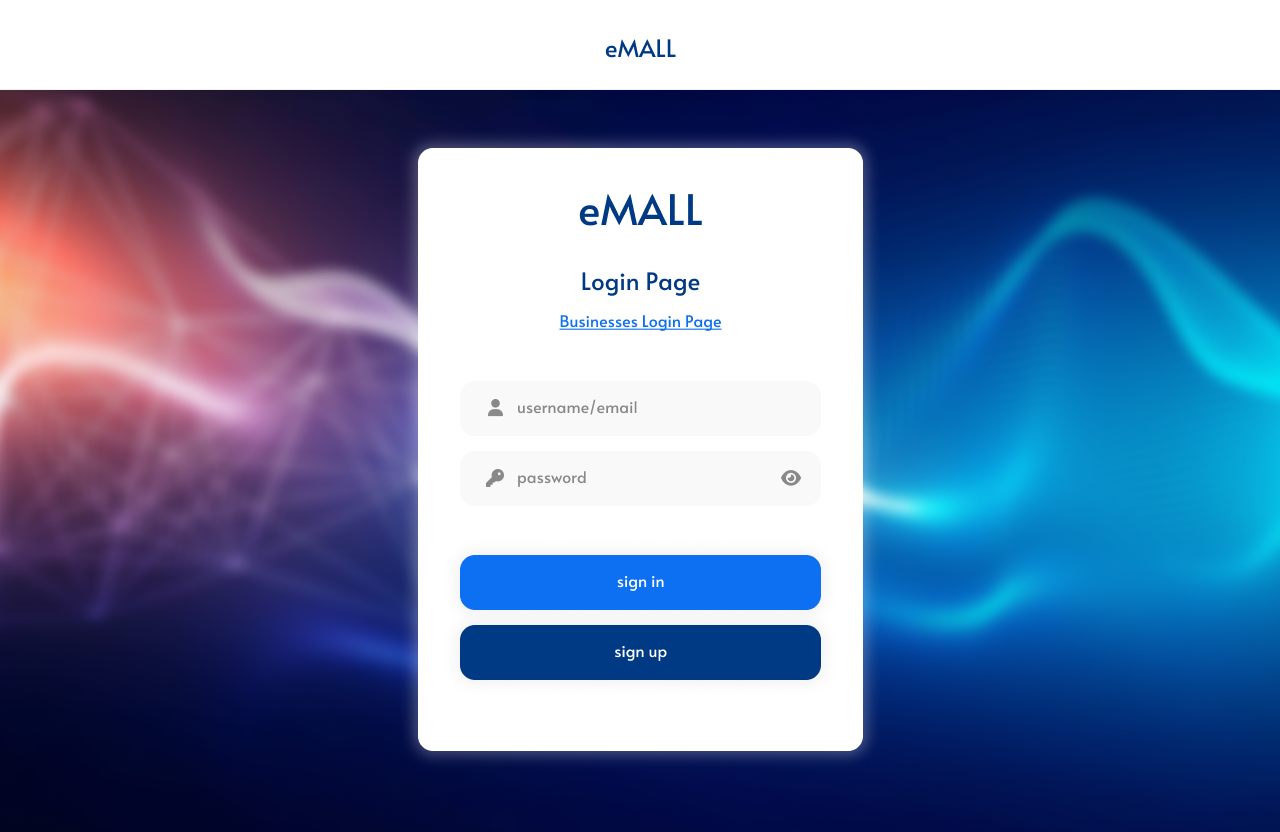
\includegraphics[width=1\linewidth]{UI/Signin}
		\caption{Login Page}
		\label{fig: cd}
	\end{center}
\end{figure}

Any interactive panels and dialogs are neglected in the development of the interface.

\begin{figure} [H]
	\begin{center}
		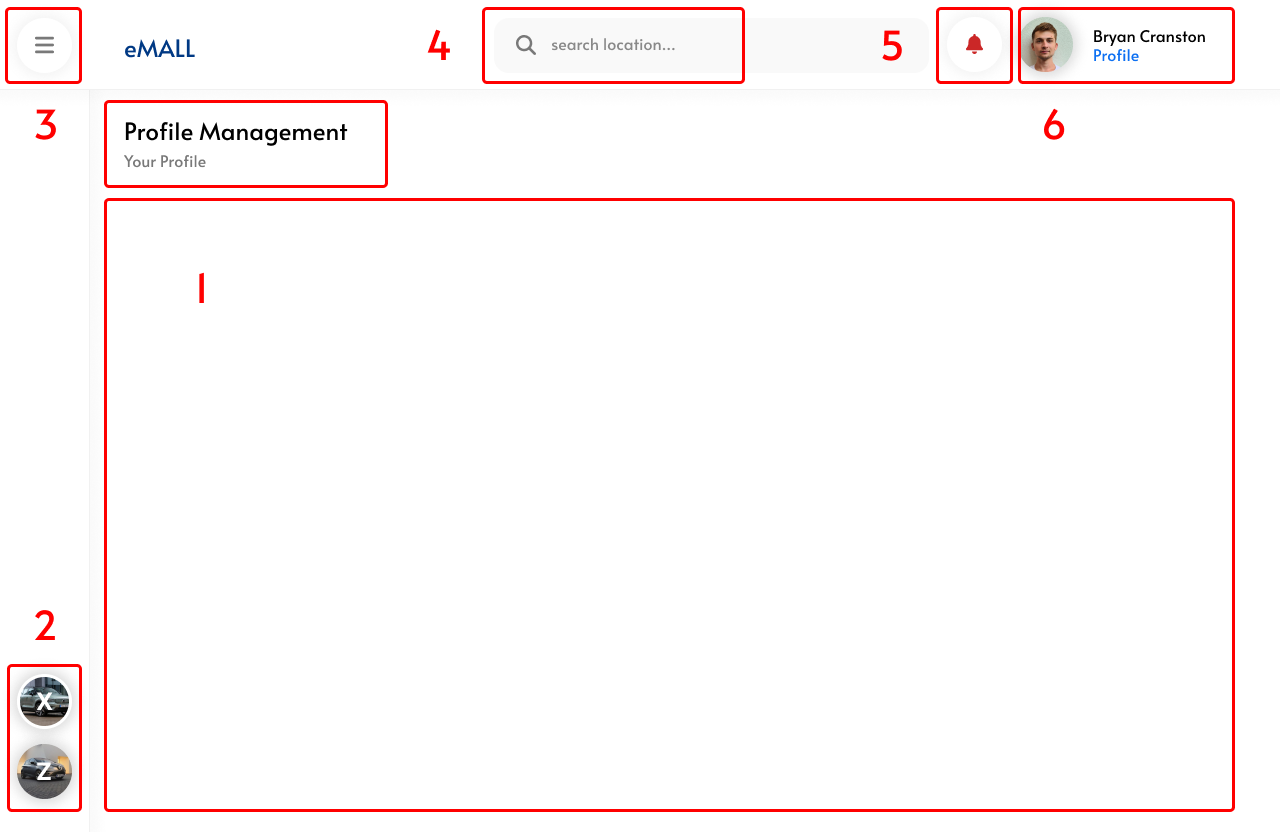
\includegraphics[width=1\linewidth]{UI/Wireframe}
		\caption{Wireframe of sticky bars}
		\label{fig: cd}
	\end{center}
\end{figure}

\begin{enumerate}
	\item \textbf{Main section:} contains the page
	\item \textbf{EV fast selector:} list buttons containing the EV owned by the user (only in the EVD dashboard), and highlights the selected EV
	\item \textbf{Hamburger toggle:} shows a menu with functions/pages offered by the system
	\item \textbf{Search bar:} permits to search a location and redirect to the map page with informations about charging stations nearby
	\item \textbf{Notification bar:} containts notifications received by the user
	\item \textbf{Profile button:} redirects to the profile page
\end{enumerate}

\section{EVD Interface}
\label{sec: evd_interface}%
The EVD dashboard collects useful informations for driver, everything at a glance. The framework is designed to be modular, which makes it versatile and responsive. The UI below contains some modules that could eventually be displayed; the dashboard is thought in particular with a section dedicated to statistics, allowing users to view their charging stats and make the system smart. 

\begin{figure} [H]
	\begin{center}
		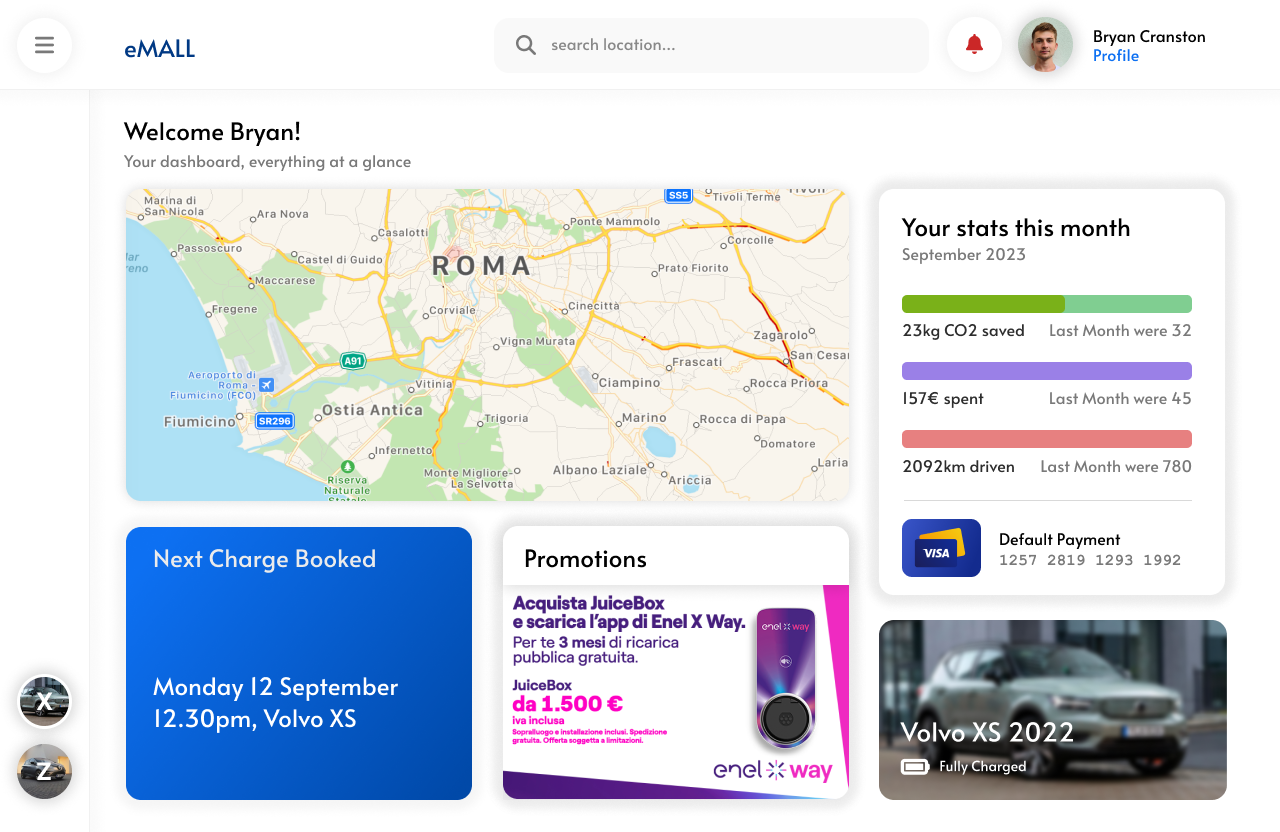
\includegraphics[width=1\linewidth]{UI/EVDDashboard}
		\caption{EVD Dashboard}
		\label{fig: cd}
	\end{center}
\end{figure}

The process of booking a charge could begin looking at the map page, which is reported below. The EVD can move around, and look for a charging stations that suits its requirements;

\begin{figure} [H]
	\begin{center}
		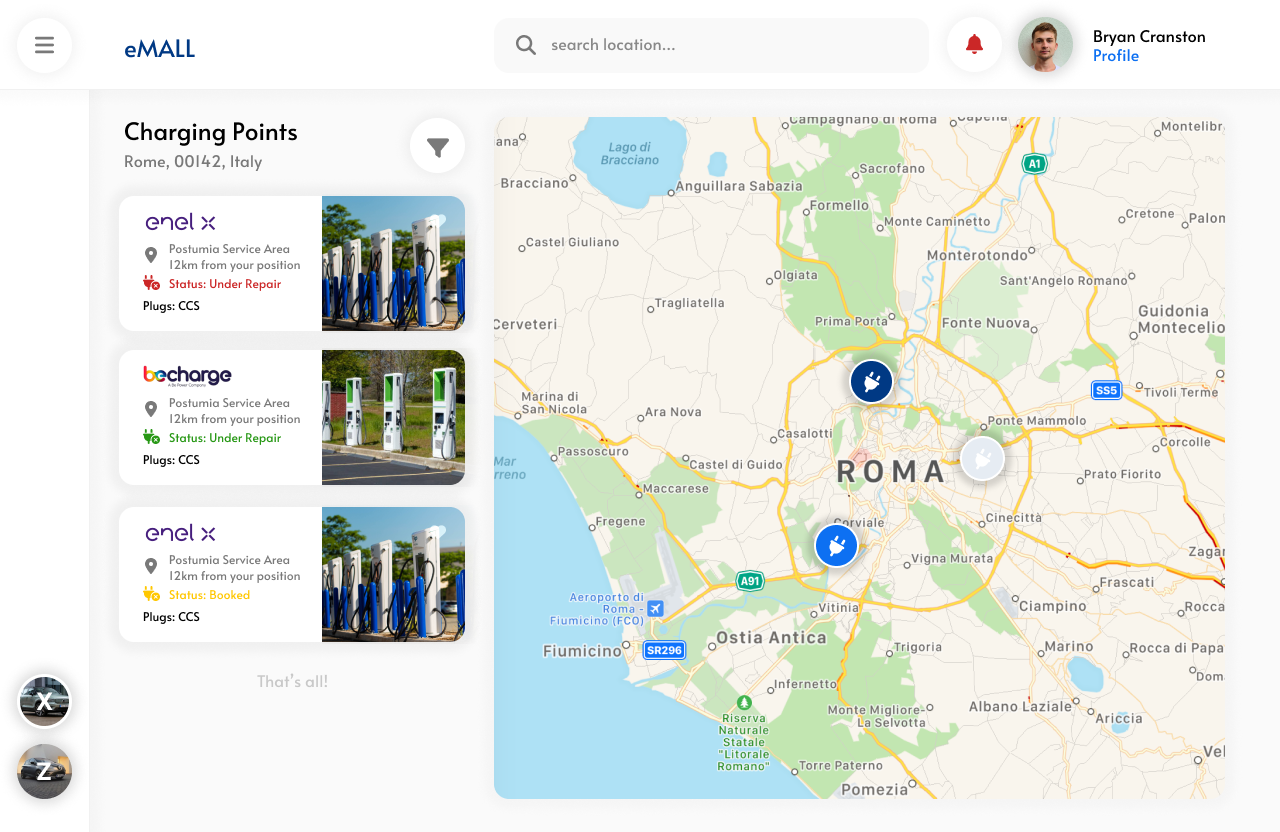
\includegraphics[width=1\linewidth]{UI/Map}
		\caption{Map page}
		\label{fig: cd}
	\end{center}
\end{figure}

Once the choice has been made, the user is redirected to the booking section, containing a calendar showing the hourly availability of the columns and their status. Some additional info about the charging stations are shown too. The charge can be booked for a specific car, and a special button is provided right below the hourly table. A user can explore the table, change dates, and confirm booking, or go back to the previous page. Lastly, the EVD can add the charging station to its favorites.

\begin{figure} [H]
	\begin{center}
		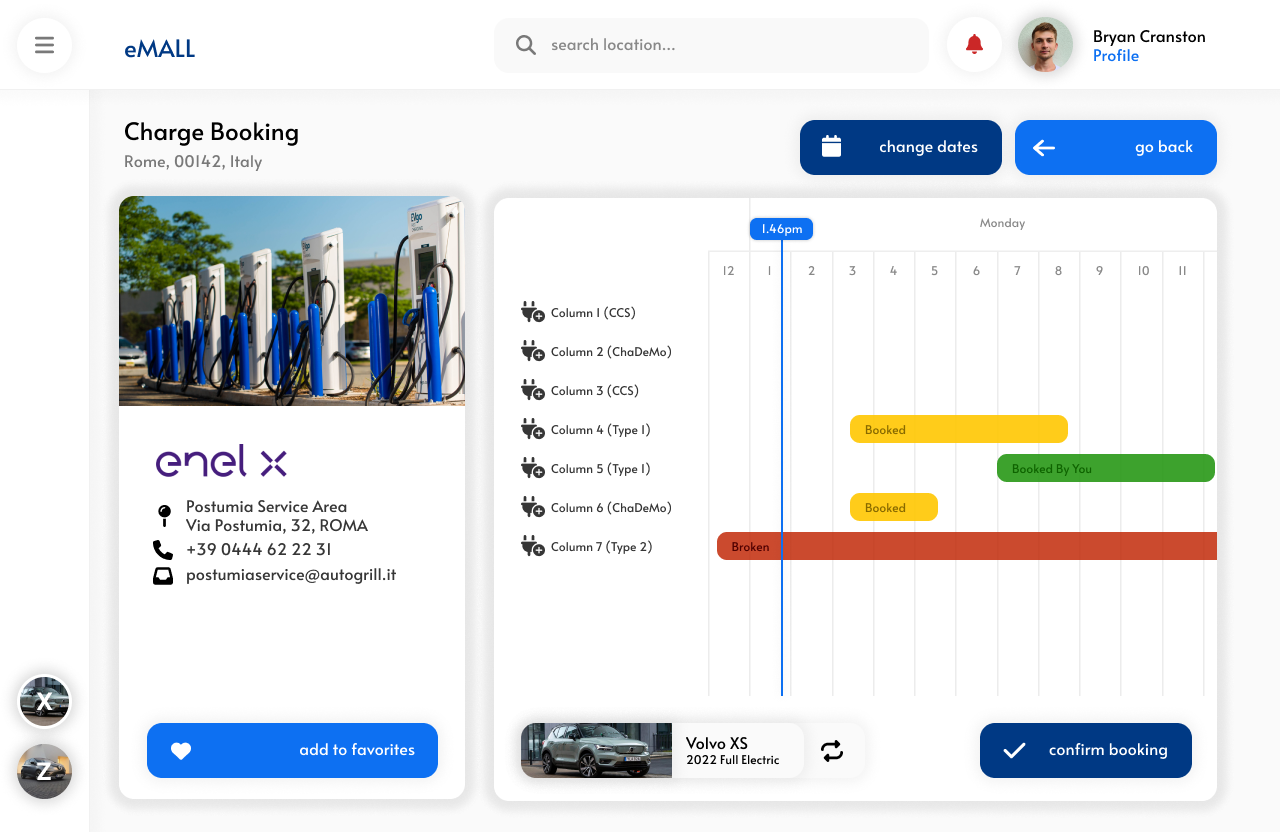
\includegraphics[width=1\linewidth]{UI/Chargebooking}
		\caption{Charge booking page}
		\label{fig: cd}
	\end{center}
\end{figure}

From the dashboard or the menu, the EVD can access to its calendar, showing its appointments, and eventually any suggested charge, based on the EVD’s habits and its EV’s necessities.

\begin{figure} [H]
	\begin{center}
		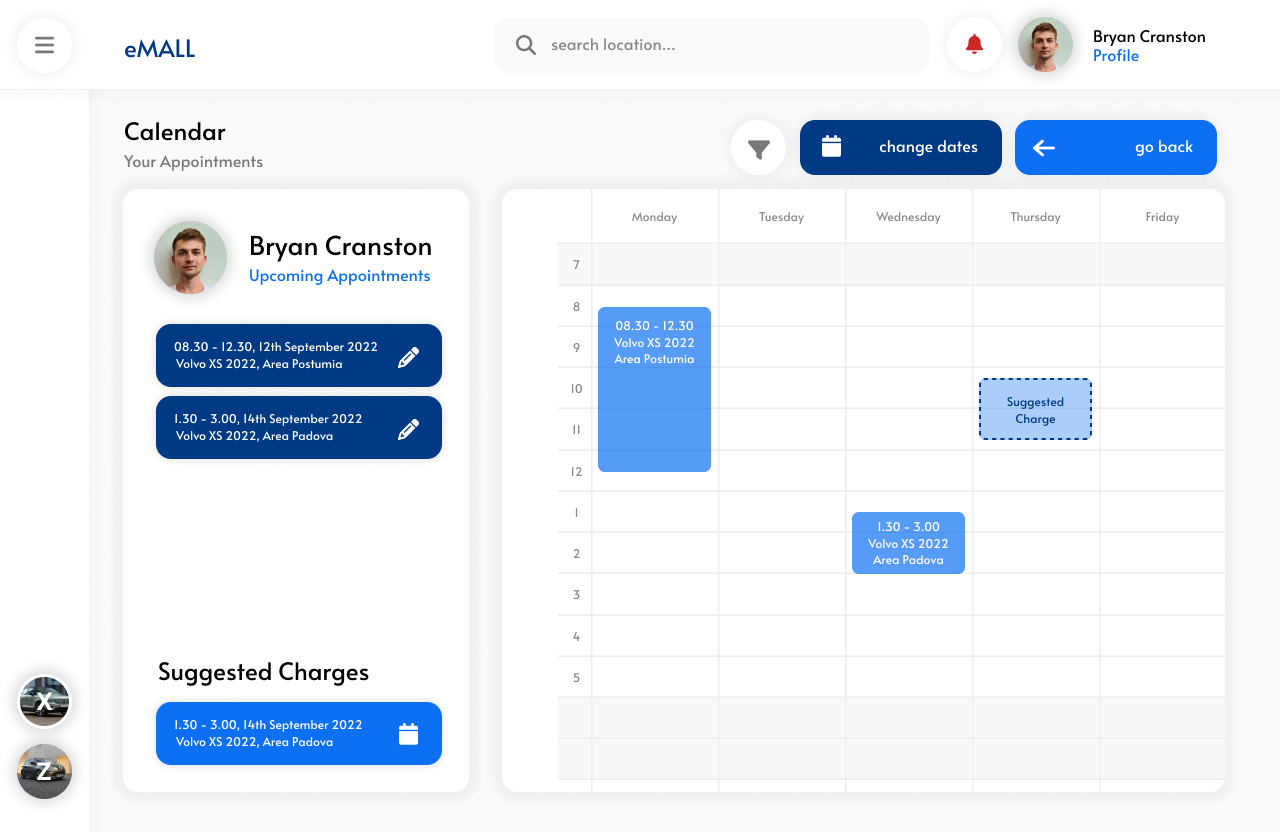
\includegraphics[width=1\linewidth]{UI/Calendar}
		\caption{Calendar page}
		\label{fig: cd}
	\end{center}
\end{figure}

A user can update its EVs’ info, add new EV or remove them in the EV mangement section.

\begin{figure} [H]
	\begin{center}
		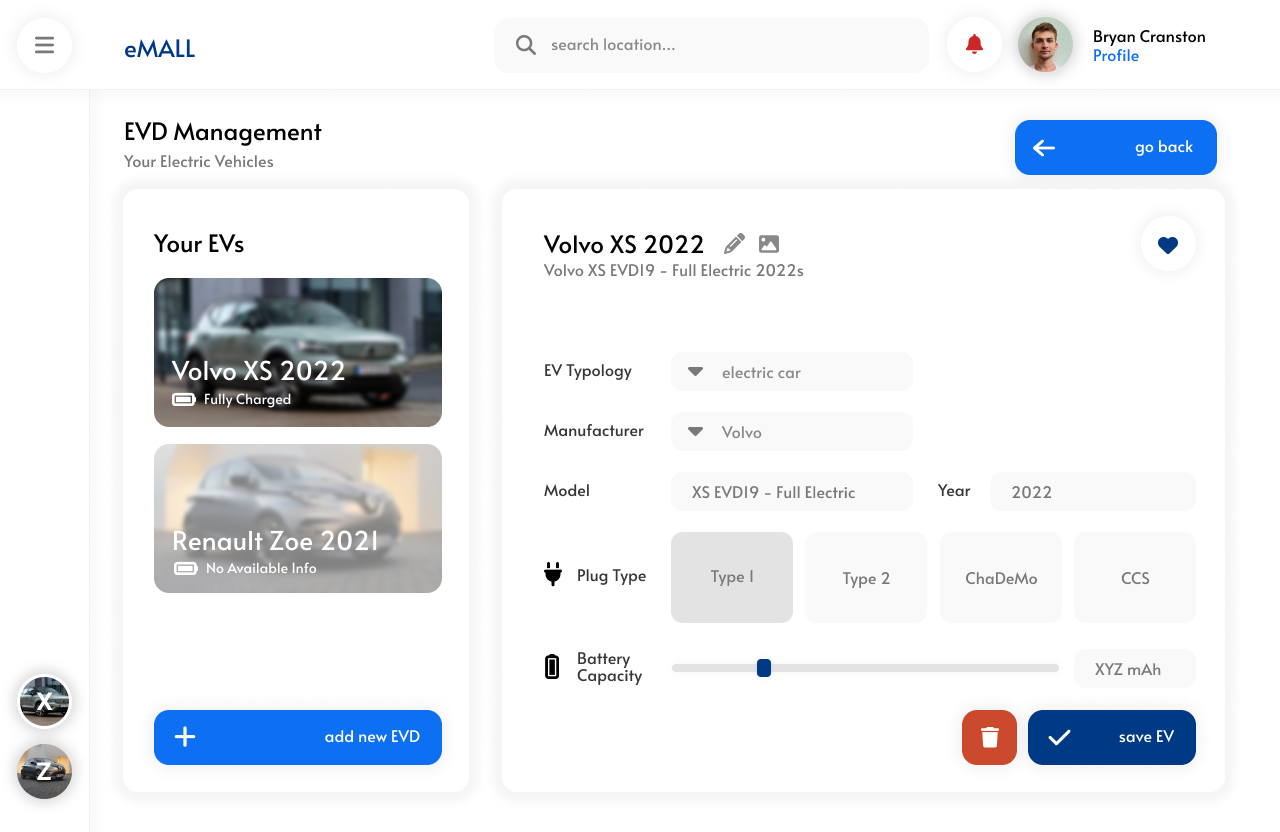
\includegraphics[width=1\linewidth]{UI/VM}
		\caption{EV Management page}
		\label{fig: cd}
	\end{center}
\end{figure}

Finally, a profile management section can be accessed from the profile button, or from the menu. It contains informations about the user, included billing address, and payment methods.

\begin{figure} [H]
	\begin{center}
		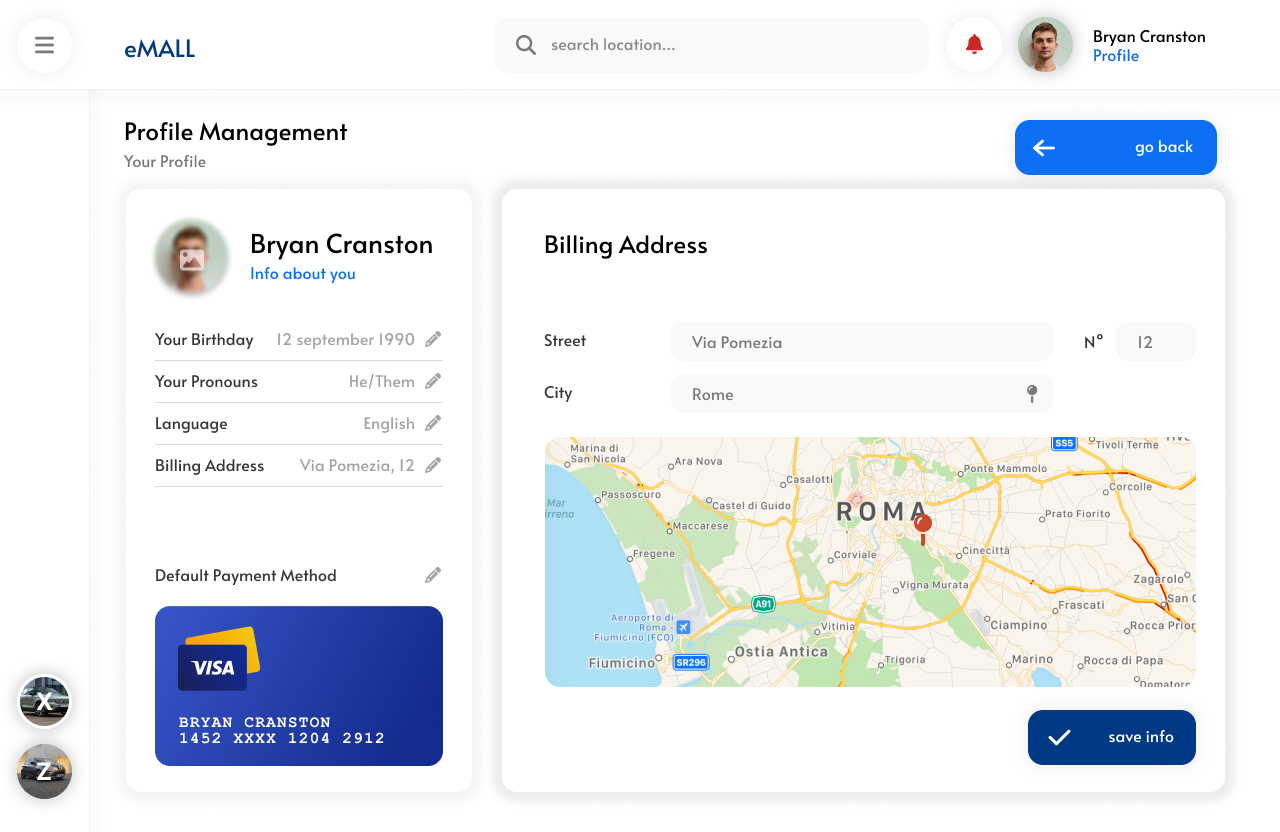
\includegraphics[width=1\linewidth]{UI/Settings}
		\caption{Settings page}
		\label{fig: cd}
	\end{center}
\end{figure}

\section{CPO Interface}
\label{sec: cpo_interface}%

The CPO’s interface is slightly different from the EVD’s interface, as said before. Offered functions and pages are the charging station management page that is shown below, containing info about its location, and the status about charging points in the selected charging station. The CPO’s operator can set fees, modify promo associated to a specific charging point, check DSO status, and finally save updated info.

\begin{figure} [H]
	\begin{center}
		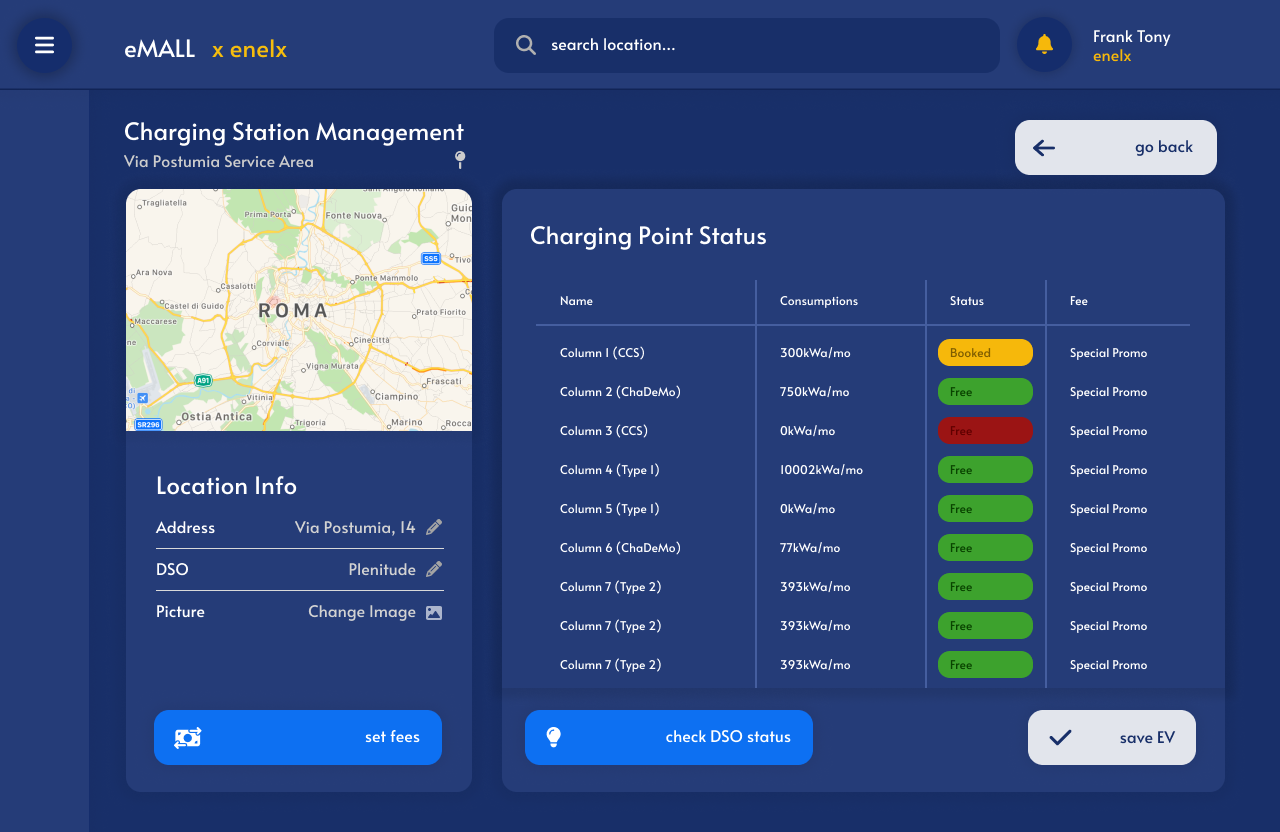
\includegraphics[width=1\linewidth]{UI/CSmgmt}
		\caption{Charging Station Management page}
		\label{fig: cd}
	\end{center}
\end{figure}

The energy acquisition page is thought to be an interface with DSOs. It displays DSO (paused, used in the past, and active); an overview is shown in the right module, containing informations about the battery/energy used; a log can be downloaded, to obtain more accurate informations. Stats about battery usage are shown in the right module too.

\begin{figure} [H]
	\begin{center}
		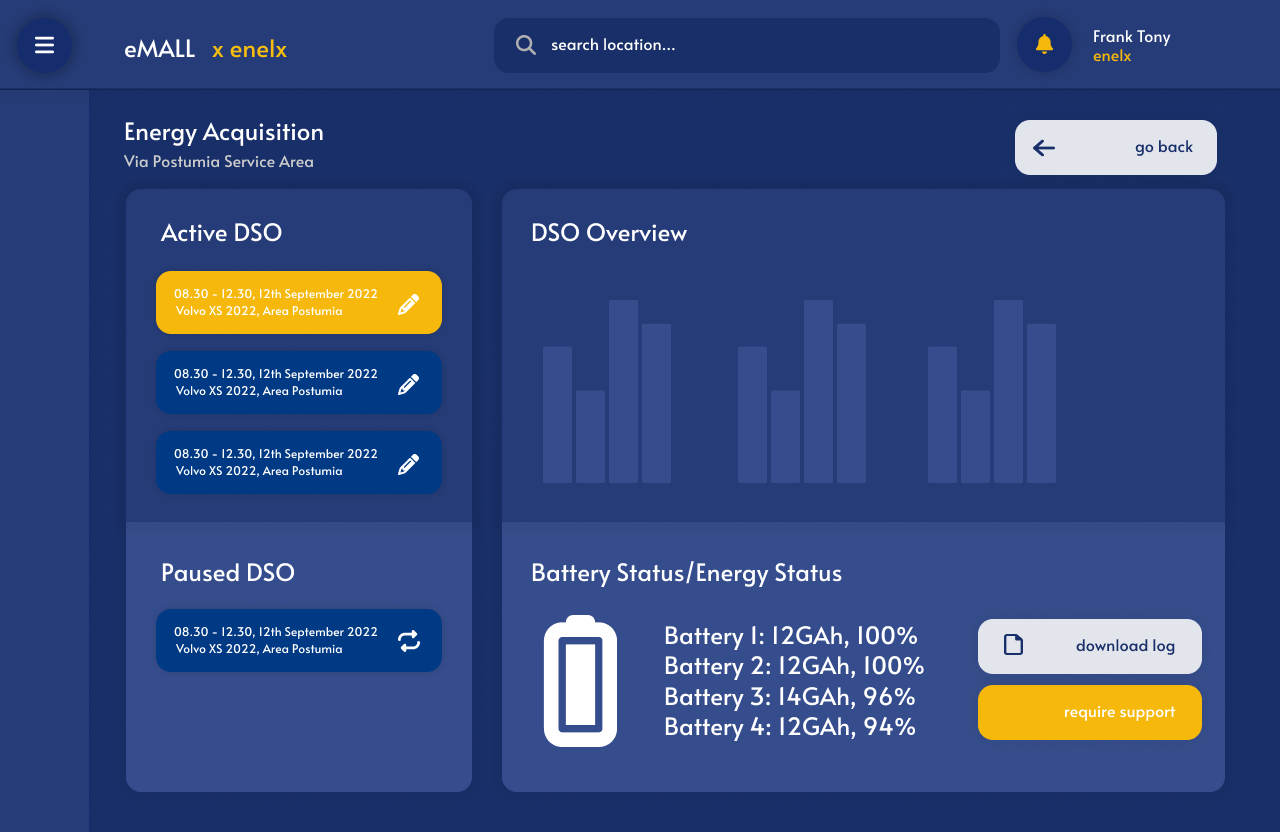
\includegraphics[width=1\linewidth]{UI/EA}
		\caption{Energy Acquisition Management page}
		\label{fig: cd}
	\end{center}
\end{figure}

Fees can be set, modified and eliminated in the fee management page.

\begin{figure} [H]
	\begin{center}
		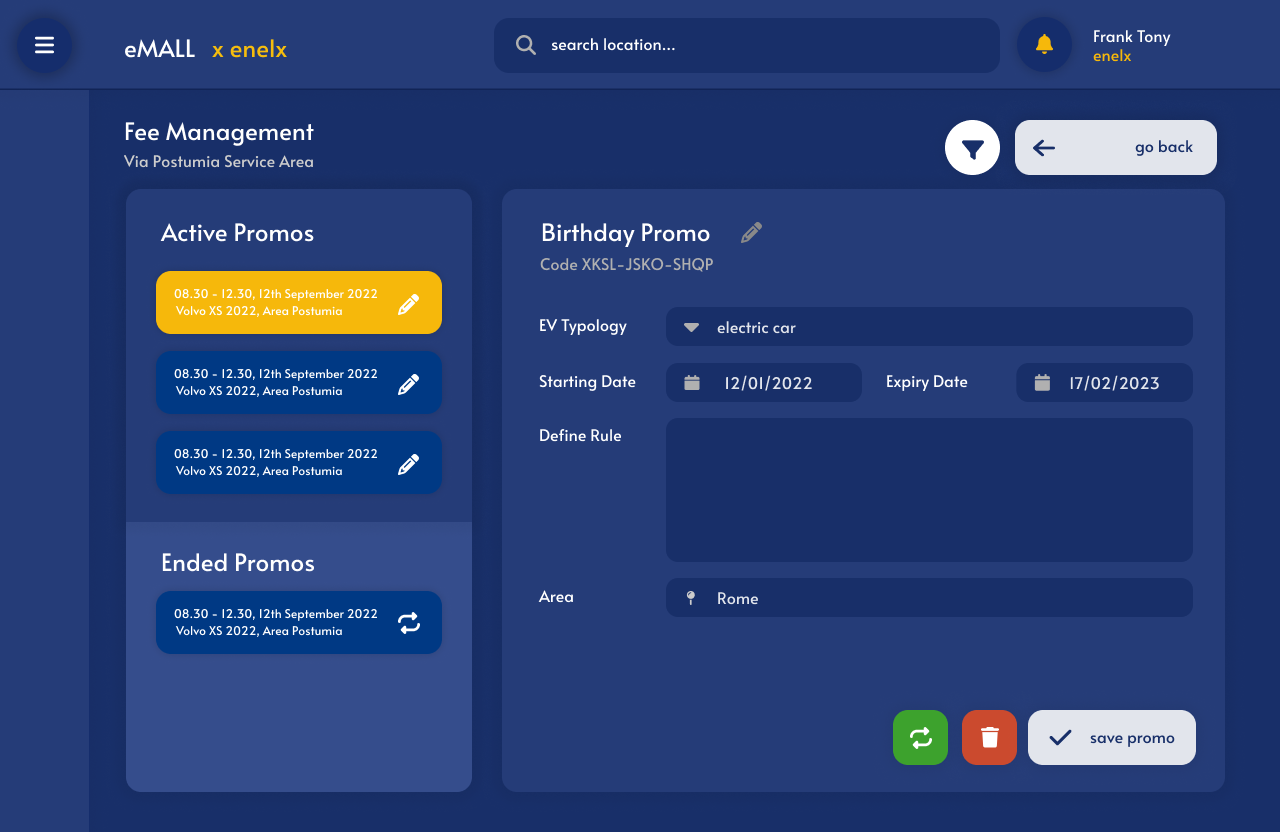
\includegraphics[width=1\linewidth]{UI/Promomgmt}
		\caption{Promo Management page}
		\label{fig: cd}
	\end{center}
\end{figure}